
\section{scNMT-seq enables joint profiling of chromatin accessibility, DNA methylation and RNA expression in single cells}

\graphicspath{{Chapter1/Figs/}}

Single-cell profiling techniques have provided an unprecented opportunity to study cellular heterogeneity at multiple molecular levels. The maturation of single-cell RNA-sequencing technologies has enabled the identification of transcriptional profiles associated with lineage diversification and cell fate commitment \cite{Kolodziejczyk2015,Griffiths2018,Papalexi2017,Patel2014}. Yet, the accompanying epigenetic changes and the role of other molecular layers in driving cell fate decisions remains poorly understood. Consequently, the profiling the epigenome at the single-cell level is receiving increasing attention, but without associated transcriptomic readouts, the conclusions that can be extracted from epigenetic measurements are limited \cite{Stuart2019,Kelsey2017,Griffiths2018}.

In this chapter we will describe scNMT-seq, an experimental protocol for genome-wide profiling of RNA expression, DNA methylation and chromatin accessibility in single cells. First, we will validate the quality of the triple omics readouts, followed by a comparison with similar available technologies. Subsequently, we will showcase how scNMT-seq can be used to reveal coordinated epigenetic and transcriptomic heterogeneity along a differentiation process.

The work discussed in this chapter results from a collaboration with the Wolf Reik lab (Babraham Institute, Cambridge, UK). It has been peer-reviewed and published in Clark \& Argelaguet et al \cite{Clark2018}.\\
The methodology was conceived by Stephen Clark, who performed most of the experiments. Felix Krueger processed and managed sequencing data. I performed the computational analysis, except for the reconsutraction of chromatin accessibility profiles, which was done by Andreas Kapourani. Guido Sanguinetti, Gavin Kelsey, John C. Marioni, Oliver Stegle and Wolf Reik supervised the project.\\
The article was jointly written by Stephen Clark, John Marioni, Oliver Stegle and Wolf Reik, and me.

\subsection{Description of the experimental protocol} \label{section:scnmt_protocol}
scNMT-seq builds upon two previous multi-modal single-cell sequencing protocols: single-cell Methylation and Transcriptome sequencing (scM\&T-seq) \cite{Angermueller2016} and Nucleosome Occupancy and Methylation sequencing (NOMe-seq) \cite{Kelly2012,Pott2016}. An overview of the experiment protocol is shown in \Cref{fig:scnmt_protocol}.

In the first step (the NOMe-seq step), cells are sorted into individual wells and incubated with a GpC methyltransferase (M.CviPI). As shown \textit{in vitro}, this enzyme labels accessible (or nucleosome depleted) GpC sites via DNA methylation\cite{Kilgore2007, Kelly2012}. In mammalian genomes, cytosine residues in GpC dinucleotides are methylated at a very low rate. Hence, after M.CviPI treatment, GpC methylation marks can be interpreted as direct read outs for chromatin accessibility, as opposed to the CpG methylation readouts, which can be interpreted as endogenous DNA methylation\cite{Kilgore2007, Kelly2012}.

In a second step (the scM\&T-seq step), the DNA molecules are separated from the mRNA using oligo-dT probes pre-annealed to magnetic beads. Subsequently, the DNA fraction undergoes single-cell bisulfite conversion\cite{Smallwood2014}, whereas the RNA fraction undergoes Smart-seq2 \cite{Picelli2014}.\\

\begin{figure}[H]
	\centering
	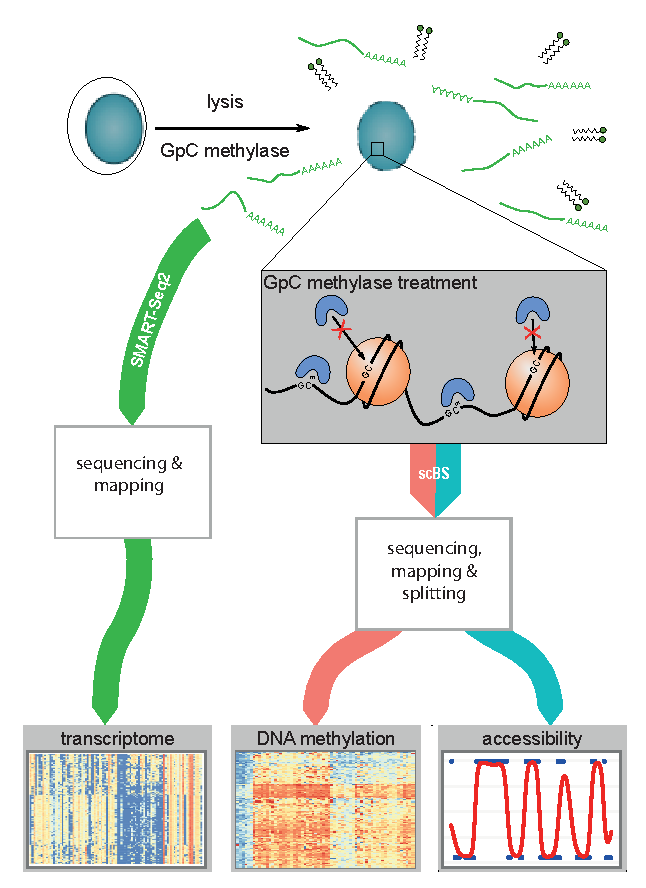
\includegraphics[width=0.6\linewidth]{scNMT_protocol}
	\caption[]{scNMT-seq protocol overview. In the first step, cells are isolated and lysed. Second, cells are incubated with a GpC methyltransferase. Third, the RNA fraction is separated using oligo-dT probes and sequenced using Smart-seq2. The DNA fraction undergoes scBS-seq library preparation and sequencing. Finally, CpG Methylation and GpC chromatin accessibility data are separated computationally.}
	\label{fig:scnmt_protocol}
\end{figure}

As discussed in \Cref{section:chromatin_accessibility}, NOMe-seq has a range of appealing properties in comparison with count-based methods such as ATAC-seq or DNAseq-seq.

First, the obvious gain of simultaneously measuring another epigenetic readout such as DNA methylation with little additional cost. Second, the resolution of the method is determined by the frequency of GpC sites within the genome ($\approx$ 1 in 16 bp), rather than the size of a library fragment (usually >100 bp). This allows the robust inspection of individual regulatory elements, nucleosome positioning and transcription factor footprints \cite{Kelly2012,Pott2016,Nordstrom2019}. Third, missing data can be easily discriminated from inaccessible chromatin. Importantly, this implies that lowly accessible sites will not suffer from increased technical variation (due to low read counts) compared to highly accessible sites. Finally, the M.CviPI enzyme shows less sequence motif biases than the DNAse or the Tn5 transposase \cite{Nordstrom2019}.
% STEPHEN: this paragraph is just copied from intro right? most of these advantages are specific to single-cell so it fits better here (i.e. i would remove a lot of this from the introduction)

The downsides of the approach are the limited scalability associated with plate-based methods, and the need to discard read outs from (1) GCG positions (21\%), as it is intrinsically not possible to distinguish endogenous methylation from \textit{in vitro} methylated bases, and (2) CGC positions (27\%), to mitigate off-target effects of the enzyme \cite{Kelly2012}. This filtering step reduces the number of genome-wide cytosines that can be assayed from 22 million to 11 million. 


\subsection{Description of the data processing pipeline}
After DNA sequencing, reads undergo quality control and trimming using TrimGalore to remove the flanking 6bp (the random primers), adaptor contamination and poor-quality base calls. Subsequently, trimmed reads are aligned to the corresponding genome assembly. Here we used Bismark \cite{Krueger2011} with the additional --NOMe option, which produces CpG report files containing only ACG and TCG trinucleotides and GpC report files containing only GCA, GCC and GCT positions. After mapping, a new round of quality control is performed based on mapping efficiency, bisulfite conversion efficiency and library size.

Finally, methylation calls for each CpG and GpC site are extracted after removal of duplicate alignments. Following the approach of \cite{Smallwood2014}, individual CpG or GpC sites in each cell are modelled using a binomial model where the number of successes is the number of methylated reads and the number of trials is the total number of reads. A CpG methylation or GpC accessibility rate for each site and cell is calculated by maximum likelihood.

When quantifying DNA methylation and chromatin accessibility rates over genomic features (i.e. promoters or enhancers), a binomial node is assumed again per cell and feature, but aggregating the counts over all CpG (methylation) and GpC (accessibility) dinucleotides overlapping the genomic feature.

\subsection{Validation}

\subsubsection{Coverage} \label{section:scnmt_coverage}
We validated scNMT-seq using 70 EL16 mouse embryonic stem cells (ESCs) cultured in serum conditions, together with two controls: negative empty wells and three cells processed without M.CviPI enzyme treatment (i.e. using scM\&T-seq). The use of this relatively simple and well-studied \textit{in vitro} system allows us to compare DNA methylation and chromatin accessibility statistics from published data \cite{Smallwood2014,Angermueller2016,Ficz2013}.

First, we compared the theoretical maximum coverage with the empirical coverage (\Cref{fig:scnmt_coverage}). Despite the reduction in theoretical coverage due to the removal of CCG and GCG sites, we observed, for DNA methylation, a median of $\approx$ 50\% of promoters, $\approx$ 75\% of gene bodies and $\approx$ 25\% of active enhancers captured by at least 5 CpGs in each cell. Nevertheless, limited coverage is indeed observed for small genomic contexts such as p300 ChIP-seq peaks (median of $\approx$ 200bp).\\
For chromatin accessibility, coverage was larger than that observed for endogenous methylation due to the higher frequency of GpC dinucleotides, with a median of $\approx$ 85\% of gene bodies and $\approx$ 75\% of promoters measured with at least 5 GpCs.

\begin{figure}[H]
	\centering
	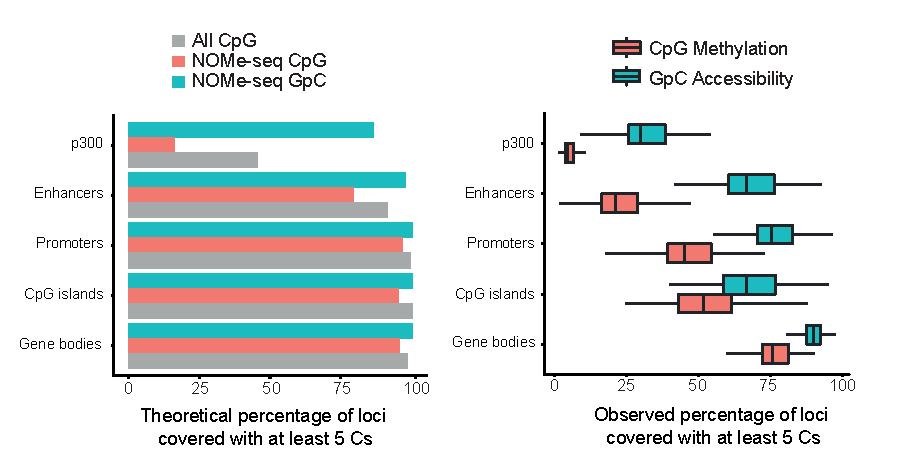
\includegraphics[width=1.0\linewidth]{scNMT_coverage}
	\caption[]{Coverage statistics for CpG DNA methylation and GpC chromatin accessibility. (a) Fraction of loci with at least 5 CpG (red) or GpC (blue) dinucleotides (y-axis) per genomic context (x-axis), after exclusion of the conflictive trinucleotides. The grey bar shows the total number of CpGs without exclusion of trinucleotides. (b) Empirical coverage (y-axis) per genomic context (x-axis) in a data set of 61 mouse ES cells. The empirical coverage is quantified as the fraction of loci with at least 5 CpG (red) or GpC (blue) observed. The boxplots summarise the distribution across cells, showing the median and the 1st and 3rd quartiles.}
	\label{fig:scnmt_coverage}
\end{figure}

Next, we compared the DNA methylation coverage with a similar data set profiled by scM\&T-seq \cite{Angermueller2016} (\Cref{fig:scnmt_coverage}), where the the conflictive trinucleotides are not excluded.\\
Despite scNMT-seq yielding less CpG measurements, we find little differences in coverage when quantifying DNA methylation over genomic contexts, albeit these become evident when down-sampling the number of reads.

\begin{figure}[H]
	\centering
	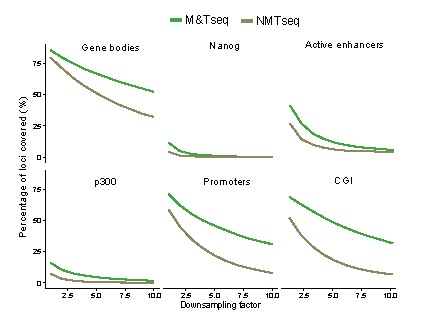
\includegraphics[width=0.8\linewidth]{scNMT_coverage2}
	\caption[]{Comparison of the empirical coverage of DNA methylation with scM\&T-seq \cite{Angermueller2016}.
	The y-axis displays the fraction of loci covered with at least 5 CpG sites. The x-axis displays the downsampling factor. To facilitate the comparison, we selected two cells that were sequenced at equivalent depth.}
	\label{fig:scnmt_coverage2}
\end{figure}

\subsubsection{Consistency with previous studies}

To assess the consistency with previous studies we performed several comparisons.

First, we computationally pseudobulked the data across all cells and we examined DNA methylation and chromatin accessibility levels at loci with known regulatory roles. We found that in promoters, DNaseI hypersensitivity sites, enhancer regions and transcription factors binding sites, DNA methylation was decreased while chromatin accessibility was increased, as previously reported \cite{Pott2016}. As a control, we observe that cells which did not receive M.CviPI treatment showed globally low GpC methylation levels ( $\approx$ 2\%, \Cref{fig:scnmt_profiles_MT}).

% TO-DO: ADD PROMOTERS
\begin{figure}[H]
	\centering
	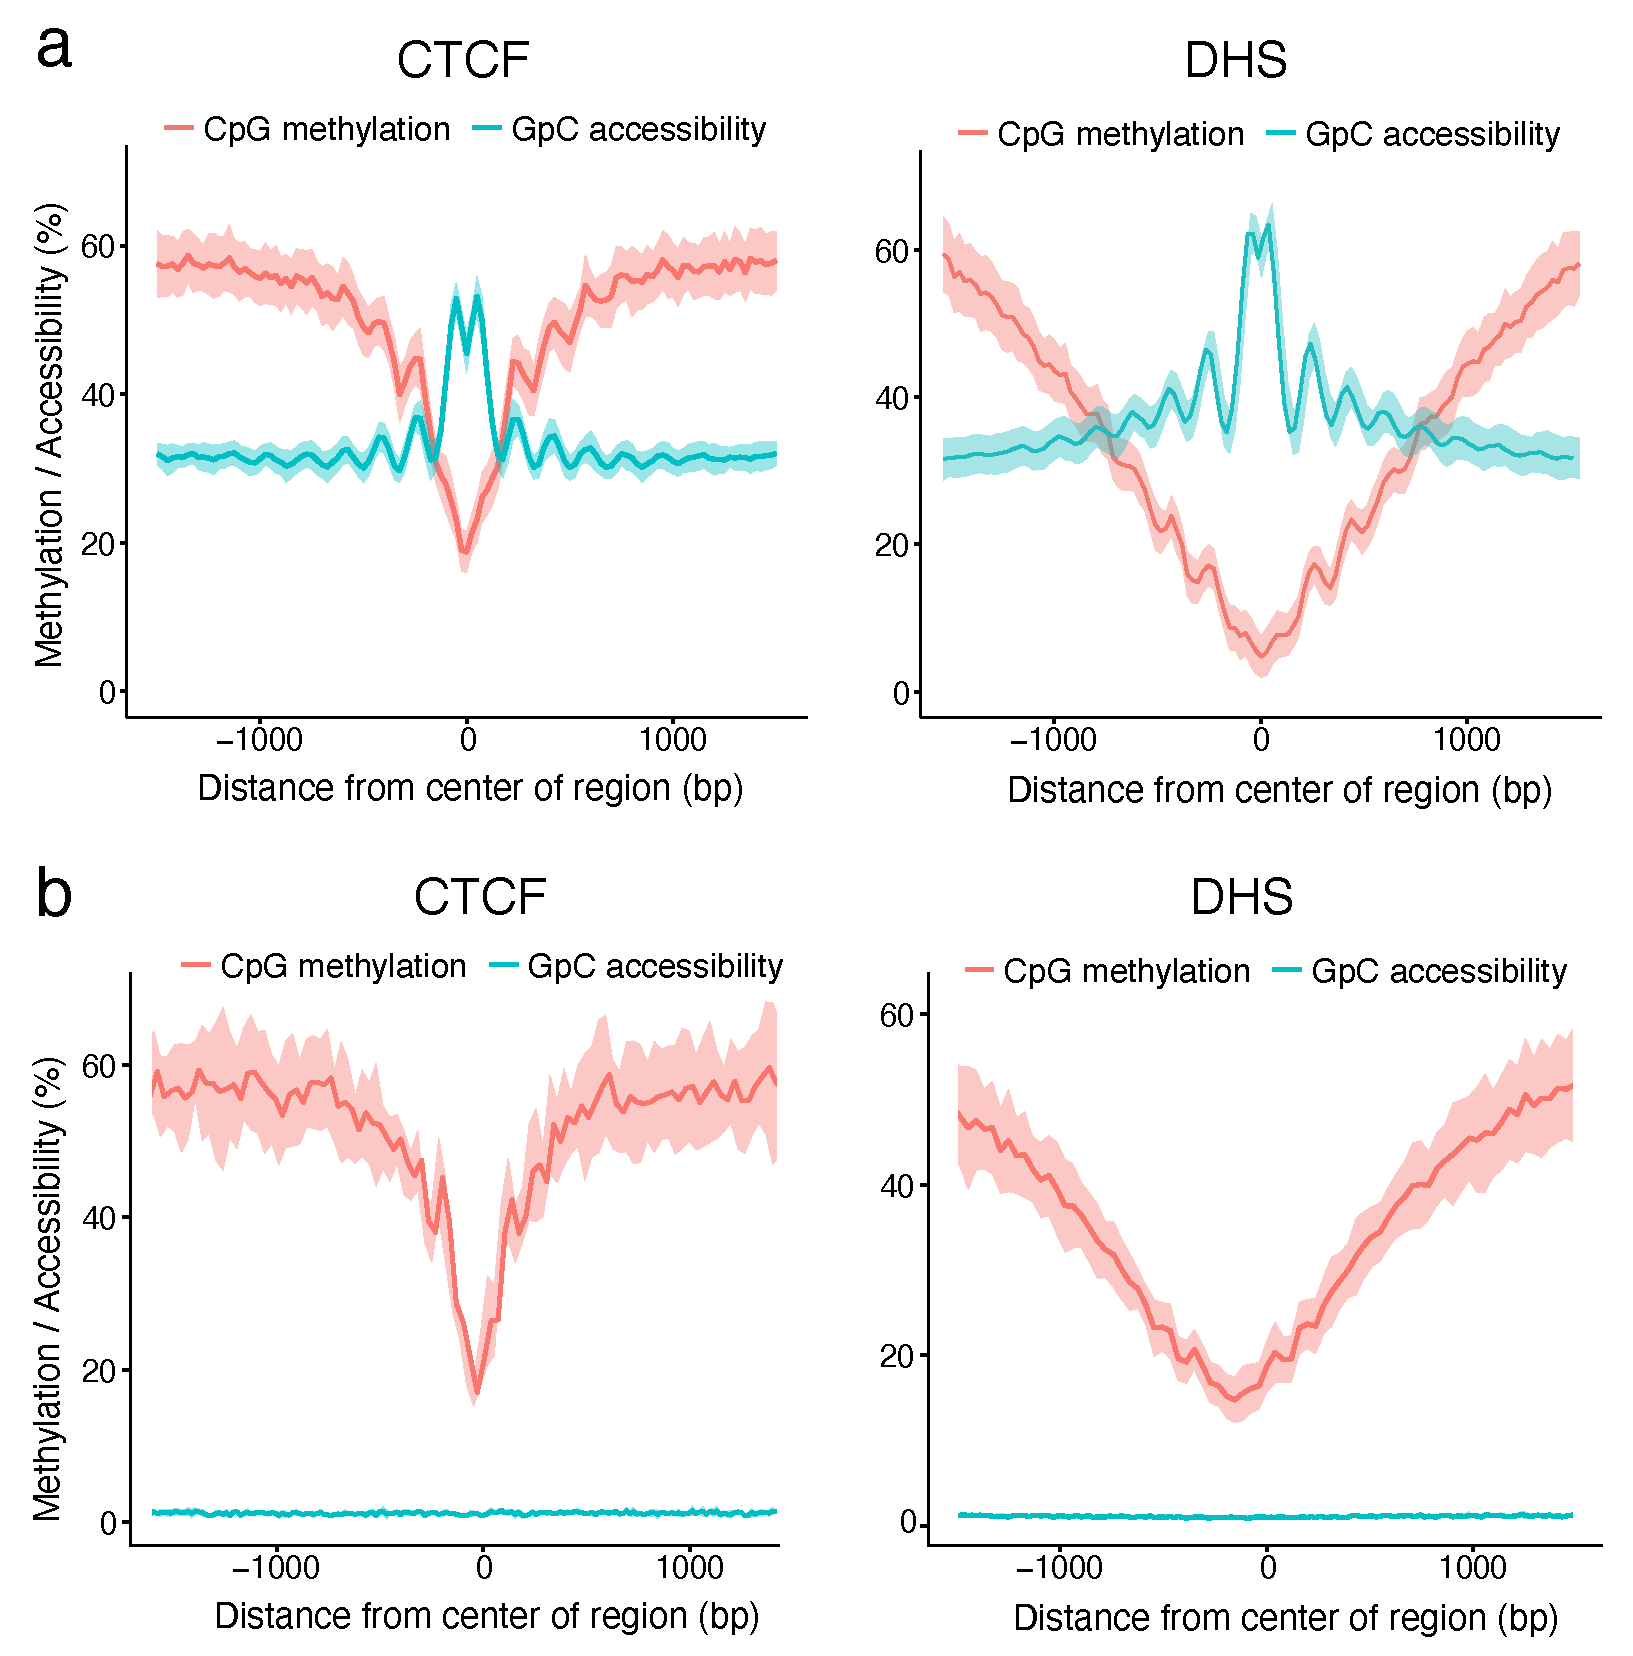
\includegraphics[width=0.8\linewidth]{scNMT_pseudobulk_profiles}
	\caption[]{Accessibility and methylation profiles in regulatory genomic contexts. First, we pseudobulk the data set by pooling information across all cells. Next, we compute running averages  of the CpG methylation (red) and the GpC accessibility (blue) in consecutive non-overlapping 50bp windows. Solid line displays the mean across all genomic elements within a given annotation and the shading displays the corresponding standard deviation.}
	\label{fig:scnmt_profiles}
\end{figure}


% TO-DO: ADD SCMT CONTROLS
% \begin{figure}[H]
% 	\centering
% 	\includegraphics[width=0.8\linewidth]{scNMT_profiles_MT}
% 	\caption[]{}
% 	\label{fig:scnmt_profiles_MT}
% \end{figure}


Second, instead of interrogating pre-defined genomic annotations, we quantified DNA methylation and chromatin accessibility using a running window throughout the genome. The resulting measurements were compared to data sets from the same cell lines profiled with similar technologies, including scM\&T-seq\cite{Angermueller2016}, scBS-seq\cite{Smallwood2014} and bulk BS-seq\cite{Ficz2013}.

When comparing the resulting methylomes, we find that most of the variation is not attributed to the technology but to differences in culture condition (serum vs 2i media). Cells grown in 2i media remain in a native pluripotency state with genome-wide DNA hypomethylation \cite{Ficz2013}, whereas cells in serum media transition to a primed pluripotency state poised for differentiation \cite{Tosolini2016}.

Interestingly, the serum-cultured cells processed in this study overlapped with 2i-cultured cells from previous data sets. suggesting that they remained in a more pluripotent state. The most likely explanation for this variation is the differences in the cell lines (we used female EL16 versus male E14 in \cite{Angermueller2016,Smallwood2014,Ficz2013}). Previous studies have sown that female ESCs tend to show lower levels of mean global methylation, which is consistent with a more pluripotent phenotype \cite{Zvetkova2005}.\\

In terms of accessibility, no NOMe-seq measurements were available for ESCs at the time of the study, so we compared it to bulk DNase-seq data from the same cell type \cite{XX}, yielding good consistency between datasets (weighted Pearson R = 0.74).
\begin{figure}[H]
	\centering
	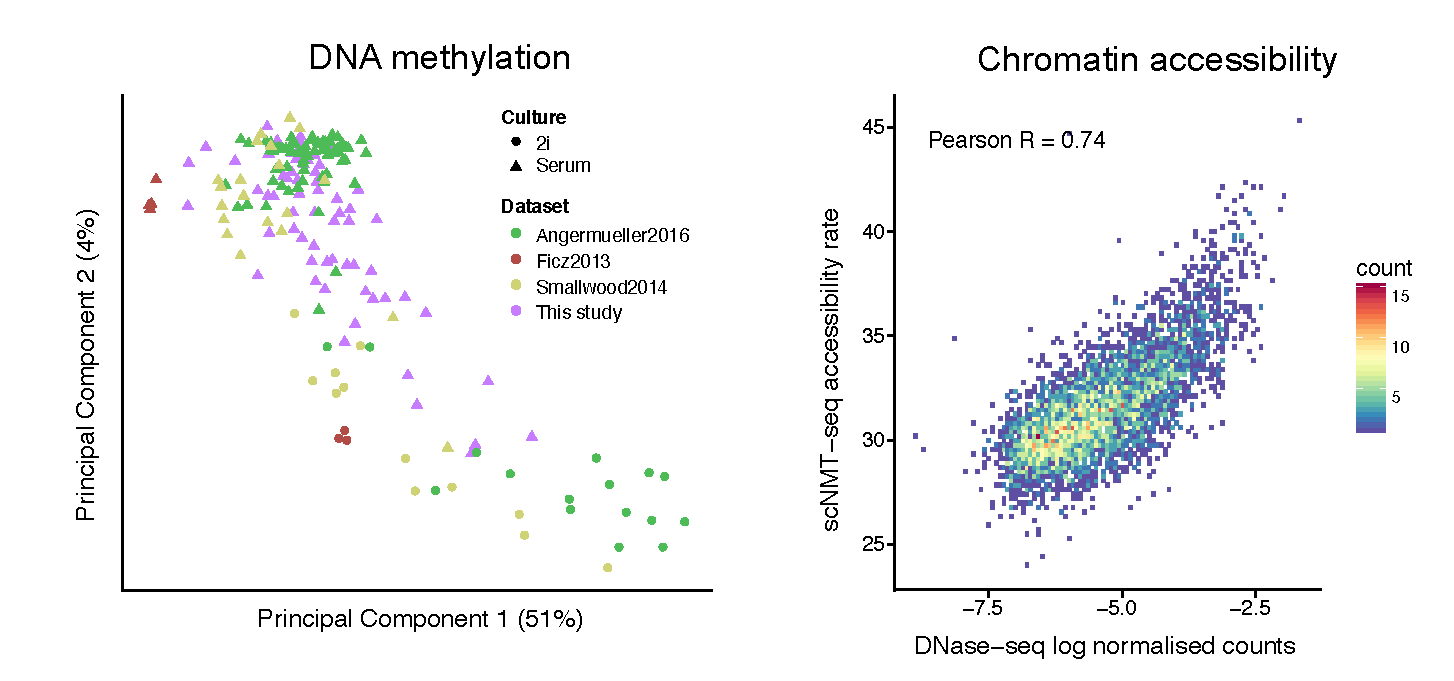
\includegraphics[width=1.0\linewidth]{scNMT_comparison}
	\caption[]{Comparison of unsupervised genome-wide quantifications to published data sets. (a) Principal Component Analysis of 1kb running windows. Missing values were imputed using the average methylation rate per locus. (b) Scatter plot of chromatin accessibility quantified over 10kb running windows of scNMT-seq data versus published bulk DNase-seq. For DNase-seq, accessibility is quantified as the log2 reads. The Pearson correlation was weighted by the GpC coverage in scNMT-seq data. }
	\label{fig:scnmt_comparison}
\end{figure}

Finally, we attempted to reconstruct the expected directional relationships between the transcriptome and the epigenome, namely the positive association between RNA expression and chromatin accessibility and the negative association between DNA methylation and RNA expression \cite{Thurman2012,Angermueller2016}.\\
To get a measure of the coupling between two molecular layers, we quantified a linear association per cell (across genes). Notice that this approach is not exclusive to single-cell data and can be computed (more accurately) with bulk measurements. Reassuringly, this analysis confirmed, even within single cells, the expected positive correlation between chromatin accessibility and RNA expression, and the negative correlations between RNA expression and DNA methylation, and between DNA methylation and chromatin accessibility.

\begin{figure}[H]
	\centering
	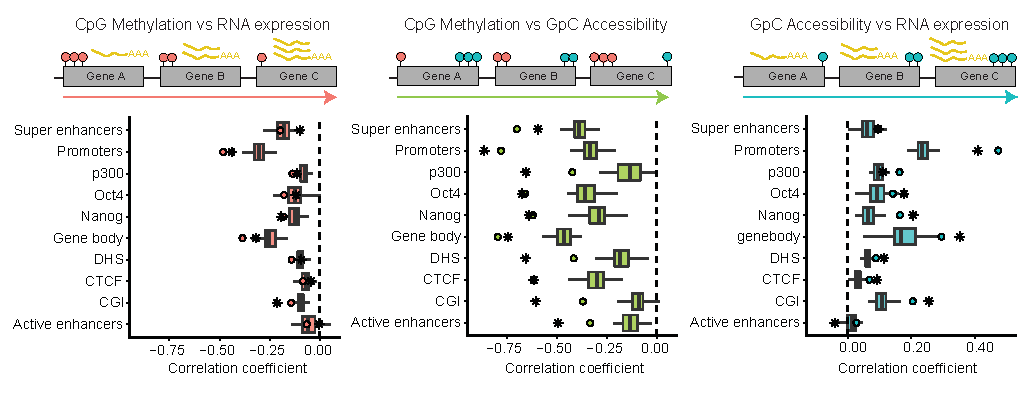
\includegraphics[width=1.0\linewidth]{scNMT_correlations_acrossgenes}
	\caption[]{Quantificaiton of linear associations between molecular layer. The top diagram illustrates the computation of an association test per cell (across all loci in a given genomic context). The left panel shows DNA methylation vs RNA expression. The middle panel shows DNA methylation vs chromatin accessibility. The right panel shows RNA expression vs chromatin accessibility. The x-axis displays the Pearson correlation coefficients between two molecular layers, per genomic context (y-axis). The box plots summarise the distribution of correlation coefficients across cells. The dots show the equivalent Pearson correlation coefficient quantified in pseudo-bulked scNMT-seq data. The stars show the same estimates using published data from the same cell types \cite{Ficz2013,ENCODE2012} }
	\label{fig:scNMT_correlations_acrossgenes}
\end{figure}

Consistently, when stratifiying the loci from \Cref{fig:scnmt_profiles} based on the expression level of the nearest gene, we observe that higher RNA expression is associated with chromatin openness and decreased DNA methylation levels. 
\begin{figure}[H]
	\centering
	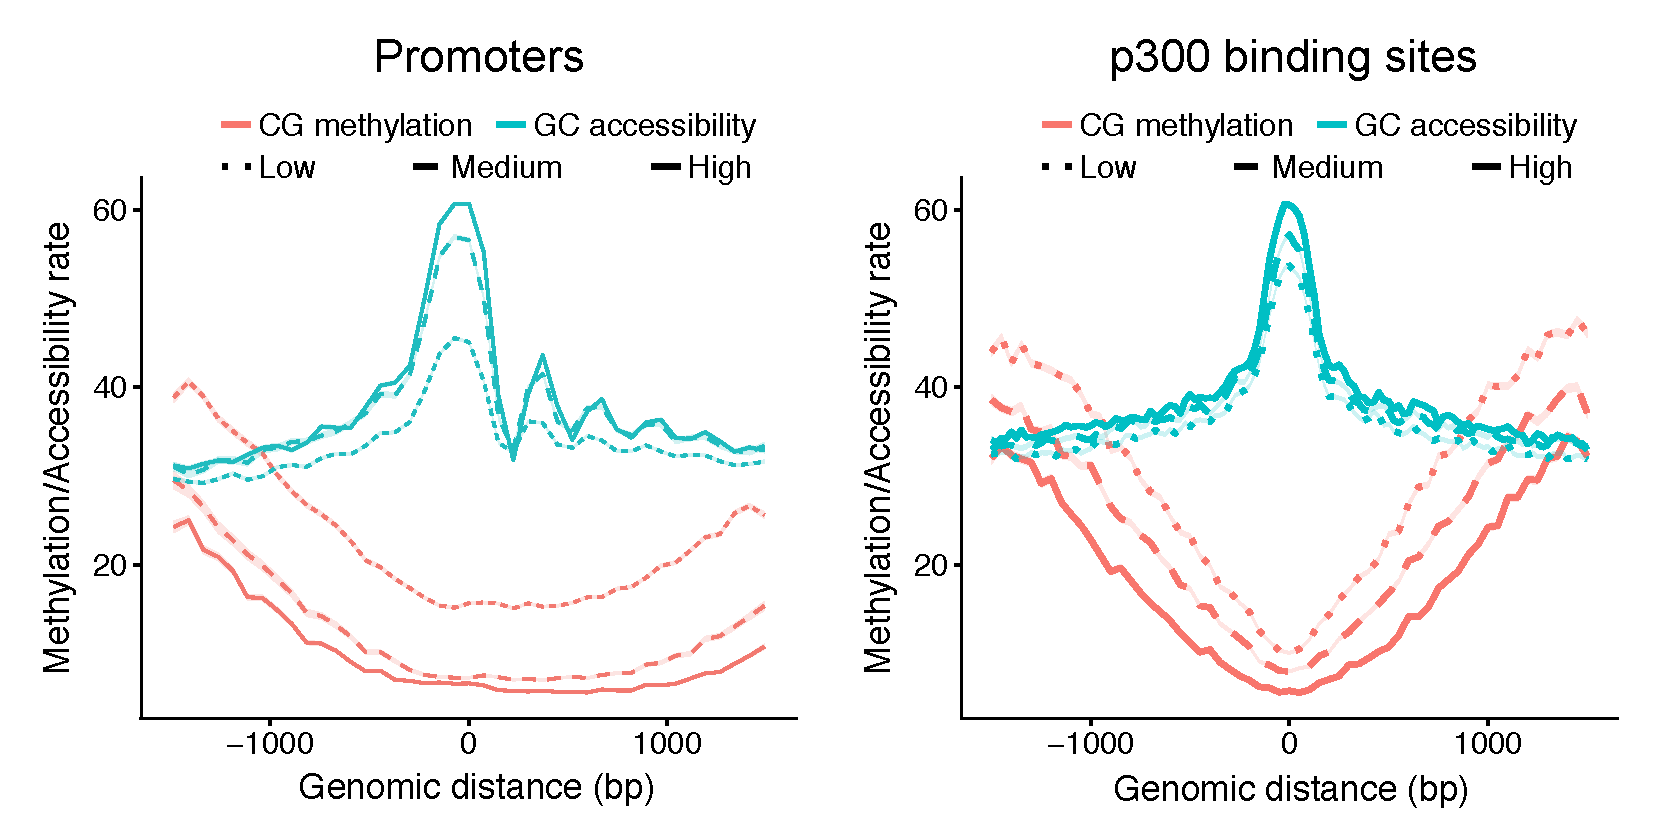
\includegraphics[width=1.0\linewidth]{scNMT_pseudobulk_profiles_byexpr}
	\caption[]{}
	\label{fig:scnmt_pseudobulk_profiles_byexpr}
\end{figure}

% Supplementary figure 4. Accessibility (blue) and methylation (red) profiles at regulatory genomic contexts, stratified by expression of the nearest gene. Shown are local GpC accessibility and CpG methylation profiles for different genomic contexts. Features are stratified by average expression level of the corresponding gene (log normalised counts less than 2 (low), between 2 and 6 (medium) and higher than 5 (high). The profile is generated by computing a running average across all cells and loci in 50bp windows.


\subsection{Identification of genomic elements with coordinated variability across molecular layers}

Having validated the quality of scNMT-seq data, we next explored its potential to identify coordinated heterogeneity across different molecular layers.\\
We generated a second data set of 43 embryonic stem cells (after QC), where we induced a differentiation process towards embryoid bodies by removing the LIF media for 3 days:

\begin{figure}[H]
	\centering
	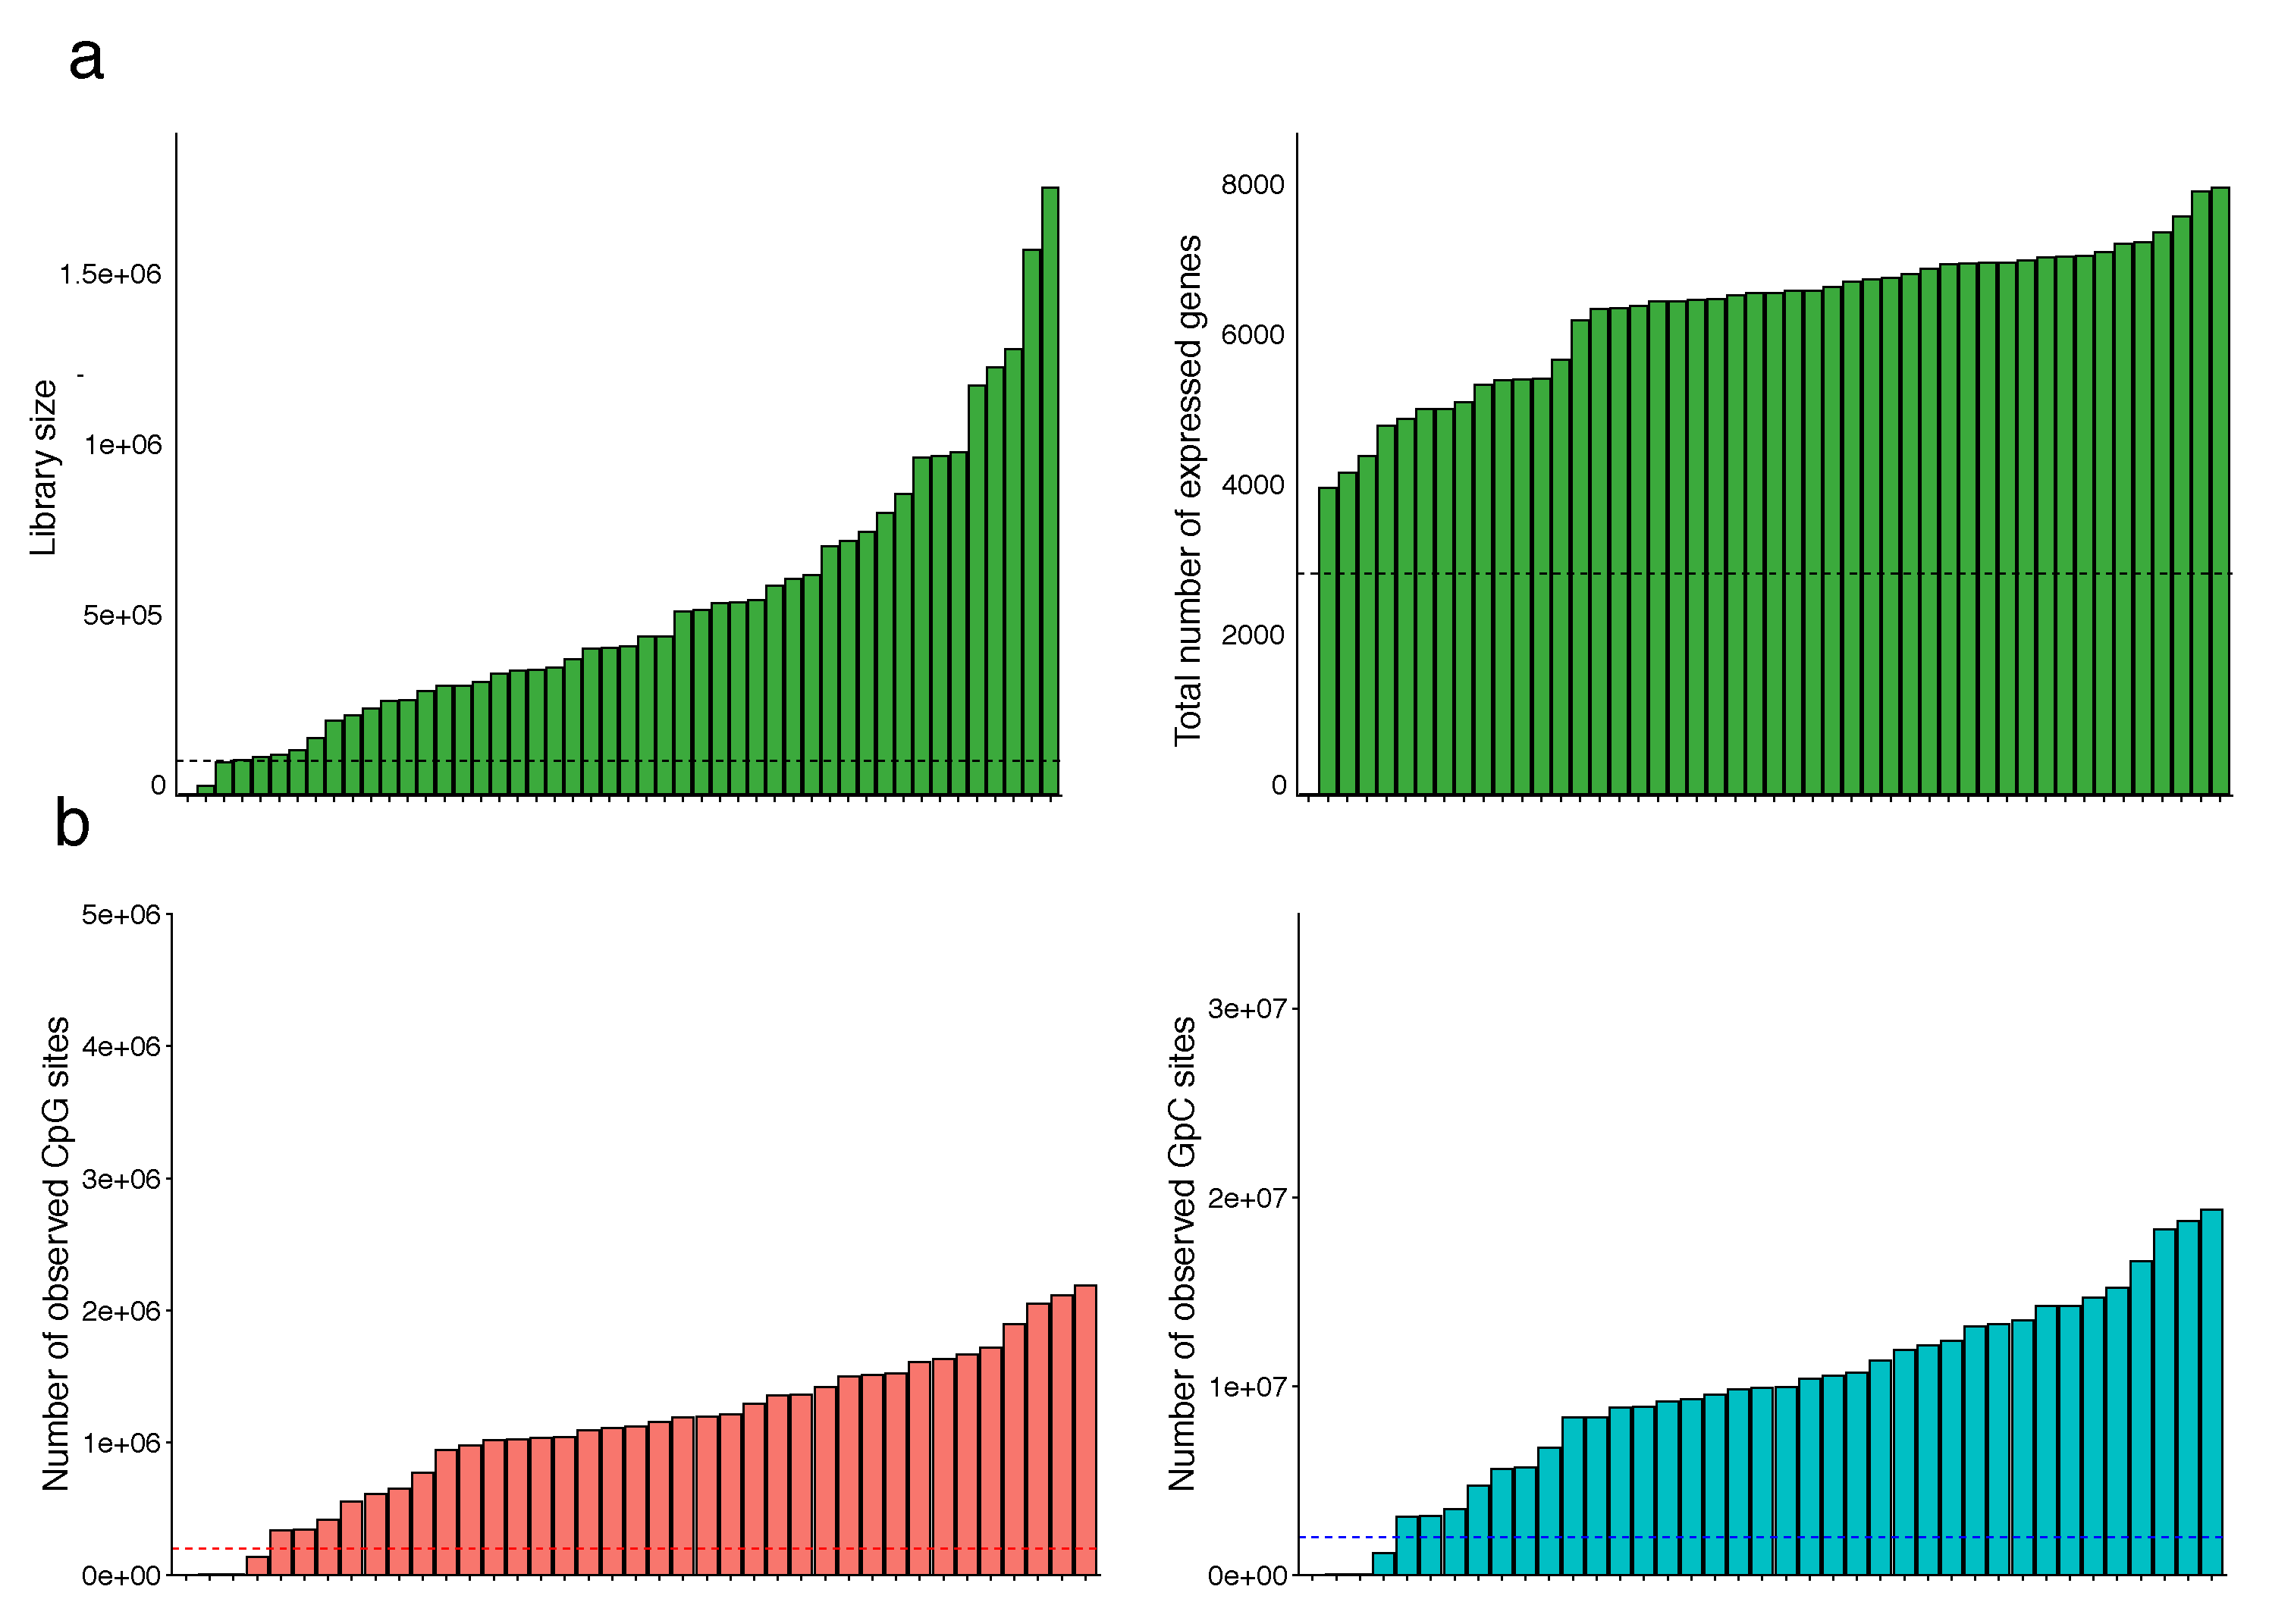
\includegraphics[width=0.8\linewidth]{scNMT_EB_QC}
	\caption[]{}
	\label{fig:scnmt_eb_qc}
\end{figure}

% displays the number of aligned reads per cell (library size) and right is the number of expressed genes (log2 normalised read counts>0) detected per cell. Cells below a set threshold (dotted lines) were removed (axis text in red).
% Displayed are the number of observed cytosine's in either CpG (left) or GpC (right) context. Cells below a set threshold (dotted lines) were removed (axis text in red).

Dimensionality reduction on the RNA expression data reveals the existence of two subpopulations: one with high expression of pluripotency markers (Esrrb and Rex1) and the other with high expression of differentiation markers (T and Prtg). This confirms the existence of significant phenotypic heterogeneity that is required for an association analysis.

\begin{figure}[H]
	\centering
	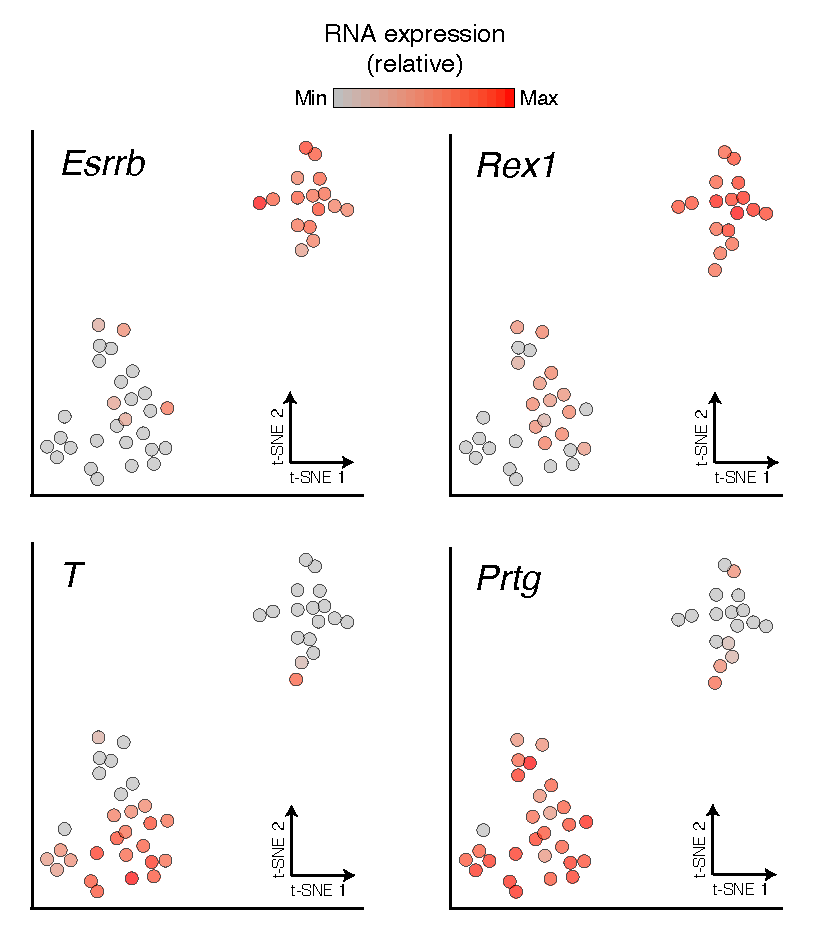
\includegraphics[width=0.8\linewidth]{scNMT_EB_RNA}
	\caption[]{}
	\label{fig:scnmt_eb_rna}
\end{figure}
% Supplementary figure 9. Visualisation of RNA-seq profiles of 43 embryoid body cells.
% Shown are bivariate visualizations using t-SNE, with expression profiles of canonical (a) pluripotency and (b) differentiation markers genes, overlaid in colour. Cells cluster into two main populations, which we subsequently labelled as pluripotent (high expression of pluripotency genes) and differentiated (low expression levels of pluripotency genes)

Next, we tested locus-specific linear associations (across cells) between pairwise combinations of molecular layers, using the average CpG rate and GpC rate within a loci as a metric for DNA methylation and chromatin accessibility, respectively.\\
First, considering correlations between DNA methylation and RNA expression, we identified a majority of negative associations, reflecting the known relationship between these two layers. In contrast, we obtained largely positive associations between chromatin accessibility and RNA expression, mainly in promoters, p300 binding sites and super enhancer regions. Finally, we found mostly negative associations between DNA methylation and chromatin accessibility, as previously reported \cite{XX}.\\
Again, this confirms the expected direction of association between molecular layers, as reported in bulk studies. Yet, the single-cell measurements allow us to inspect the dynamics of single loci (across cells). As an illustrative example, we display the Estrogen Related Receptor Beta (Esrrb) locus, a gene involved in early development and pluripotency \cite{Papp2012}. A previous study \cite{Angermueller2016}, identified a super enhancer near Esrrb that showed high degree of correlation between DNA methylation and associated RNA expression changes. In our study, we find Esrrb to be expressed primarily in the pluripotent cells, consistent with its role in early development. When examining the epigenetic dynamics of the corresponding super enhancers, we observe a strong negative correlation between DNA methylation and RNA expression, hence replicating previous findings. Additionally, we observe a strong negative relationship between DNA methylation and chromatin accesibility, indicating the two epigenetic layers are tightly coupled, consistent with the correlations per cell (across genes), displayed in Figure X.

\begin{figure}[H]
	\centering
	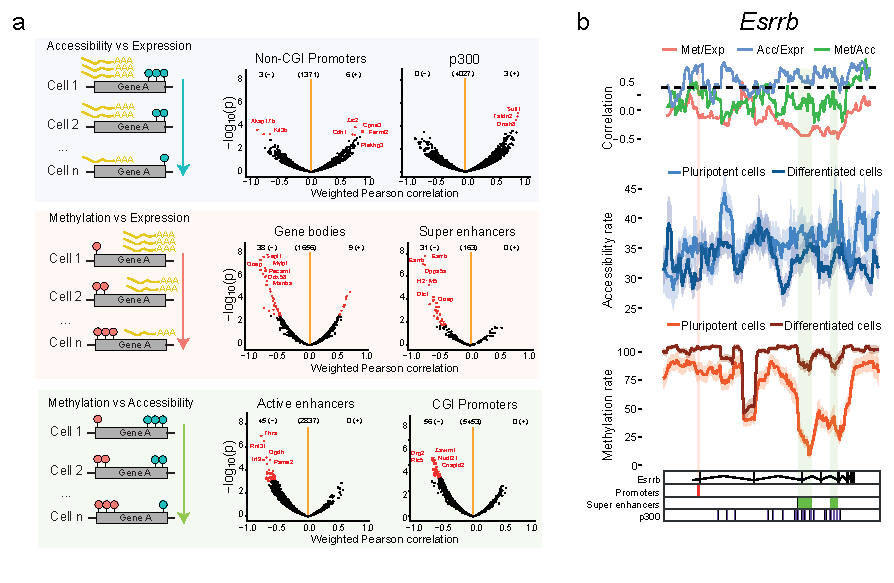
\includegraphics[width=0.9\linewidth]{scNMT_EB_correlations}
	\caption[]{}
	\label{fig:scnmt_eb_correlations}
\end{figure}

% Figure 3: scNMT-seq enables the discovery of novel associations at individual loci. (a) Left panel shows an illustration for the correlation analysis across cells, which results in one association test per locus. The right panel shows the Pearson correlation coefficient (x-axis) and log10 p-value (y-axis) from association tests between different molecular layers at individual loci, stratified by genomic contexts. Significant associations (FDR<0.1, Benjamini-Hochberg adjusted), are highlighted in red. The number of significant positive and negative associations and the number of tests (centre) are indicated above. (c) Zoom-in view of the Esrrb gene locus. Shown from top to bottom are: Pairwise Pearson correlation coefficients between each pair of the three layers (Met, methylation; Acc, accessibility; Expr, expression). Accessibility (blue) and methylation (red) profiles shown separately for pluripotent and differentiated sub-populations; mean rates (solid line) and standard deviation (shade) were calculated using a running window of 10kb with a step size of 1000bp; Track with genomic annotations highlighting the position of regulatory elements: promoters, super enhancers, and p300 binding sites

\subsection{Inference of non-linear chromatin accessibility profiles at single nucleotide resolution}
A clear advantage of scNMT-seq, compared to other chromatin accessibility technologies, is the high resolution of the its readouts, namely a binary output for each observed GpC dinucleotide. As illustrated in Figure 1, GpC accessibility measurements show complex oscillatory patterns, likely due to presence of nucleosomes, which are not appropriately captured by using an average rate. Therefore, we next attempted to exploit this high-resolution information to infer non-linear chromatin accessibility profiles at individual promoters.\\
(EXPLAIN BETTER) The approach we followed is based on BPRMeth \cite{Kapourani2018}, a generalized linear regression model with gaussian basis functions, coupled with a Bernoulli likelihood. A model was fit for every gene and every cell, provided enough coverage (at least 10 GpC sites observed per gene across 40\% of cells).\\
 Examples of infered regression patterns are shown in Figure X, showing significant heterogeneity in both the position and the number of nucleosomes:

\begin{figure}[H]
	\centering
	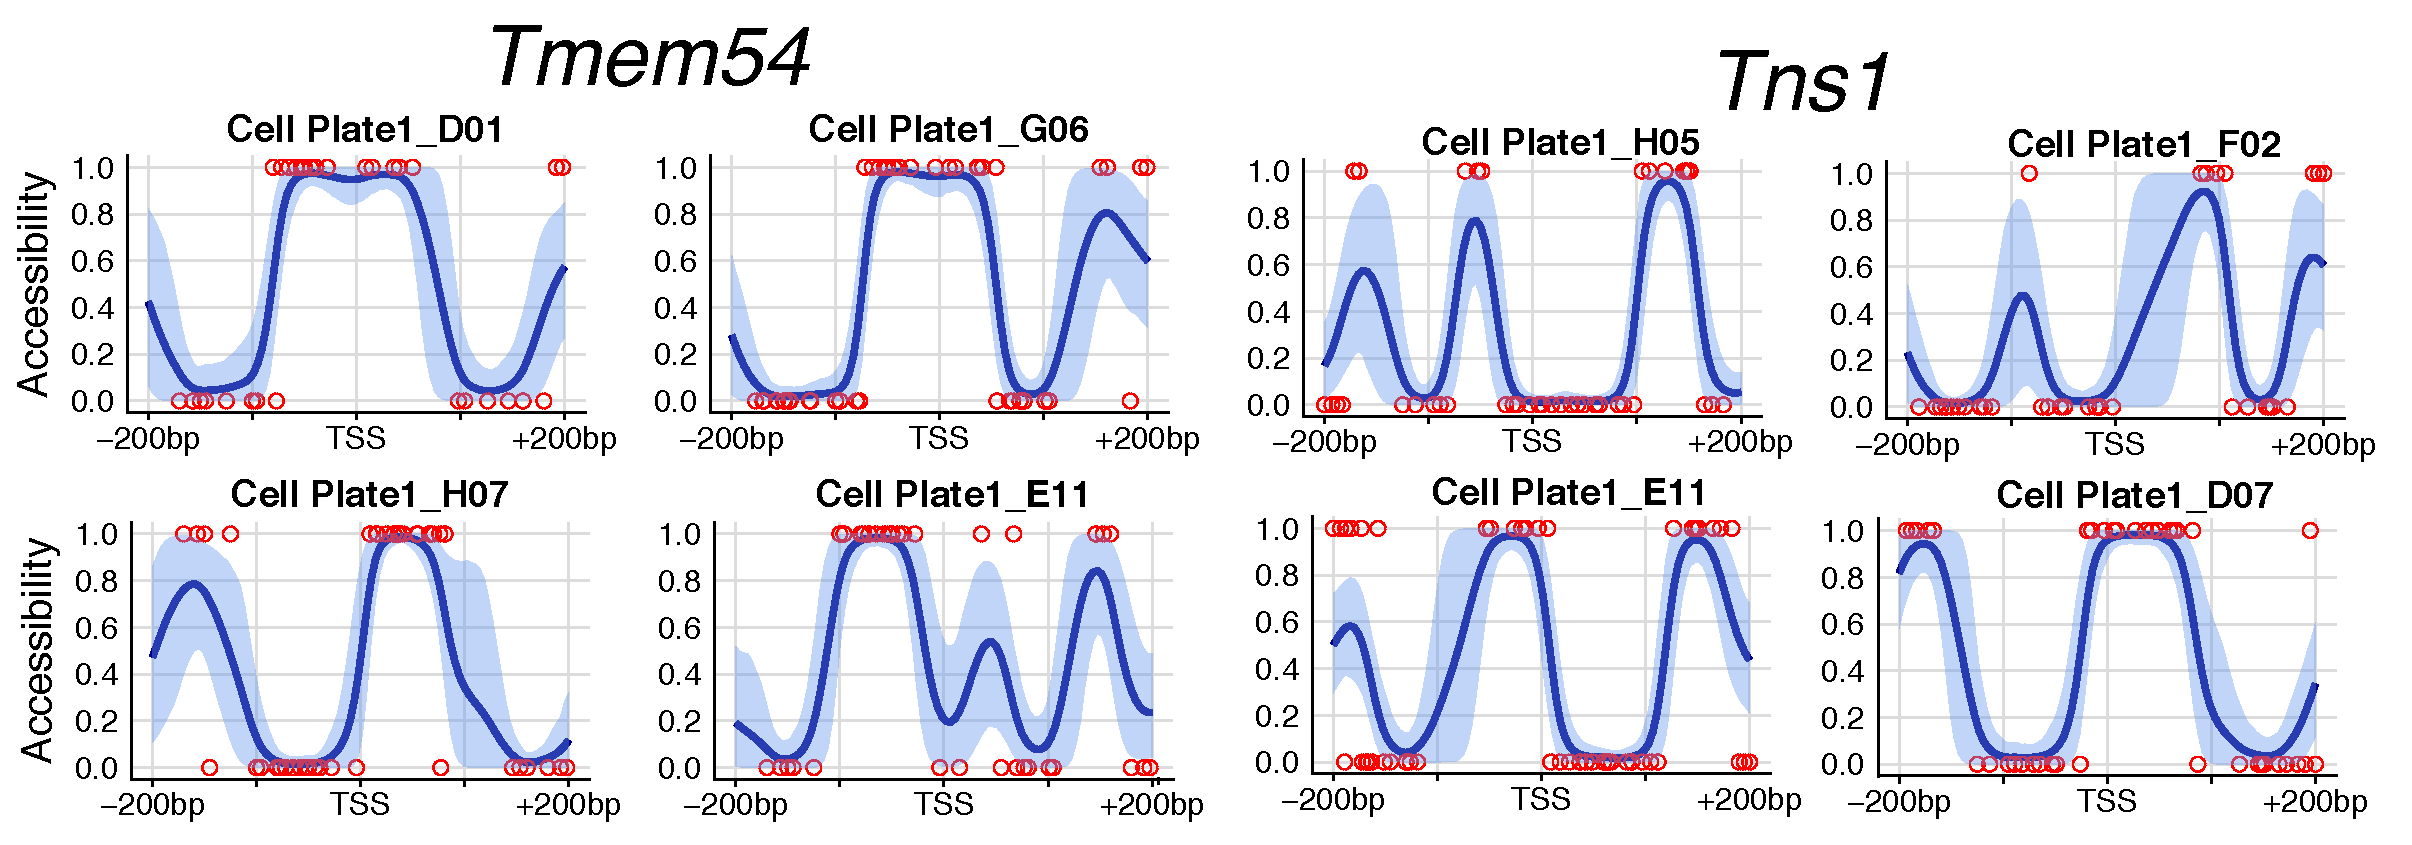
\includegraphics[width=0.9\linewidth]{scNMT_profiles_examples}
	\caption[]{}
	\label{fig:scnmt_profiles_examples}
\end{figure}

% Supplementary figure 14. Example of single-cell accessibility profiles at transcription start sites. Shown are profiles generated from four arbitrary cells in two example genes, (a) Tmem54 and (b) Tns1. Each red dot represents a GpC site, with binary accessibility value (1=accessible, 0=inaccessible). Blue line represents the mean of the posterior distribution of the inferred non-linear function, and the shading represents the corresponding 80% credible interval. Inference was done using the BPRMeth package5. Axis ticks display windows of +- 200bp around the TSS. We observe periodic patterns in the GC accessibility data, which likely indicate positions of nucleosomes

As a first validation step, we showed that the accessibility profiles infered around the transcription start site (TSS) lead to a better prediction of RNA expression than using conventional accessibility rates (Figure X).

\begin{figure}[H]
	\centering
	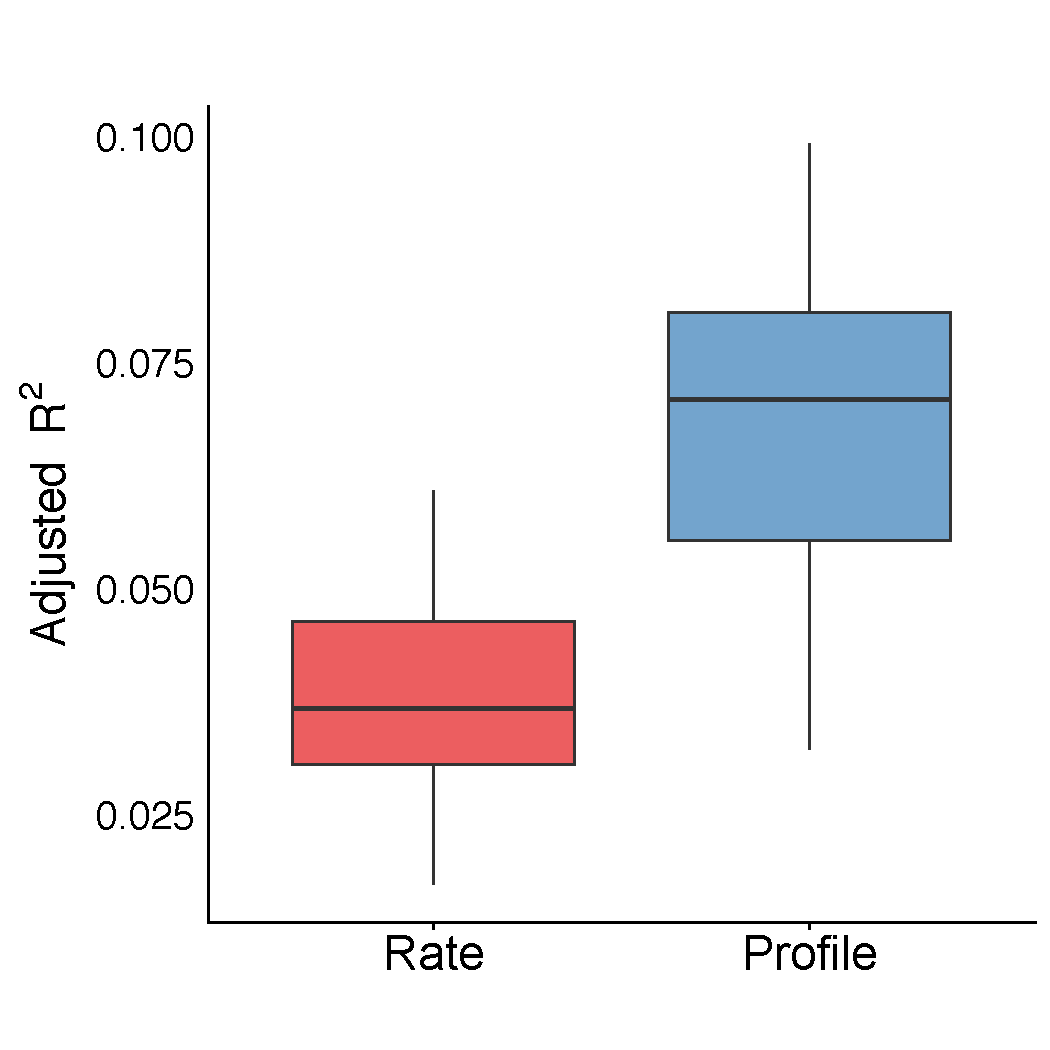
\includegraphics[width=0.65\linewidth]{scNMT_profiles_prediction}
	\caption[]{}
	\label{fig:scnmt_profiles_prediction}
\end{figure}
% Supplementary Figure 13. Accessibility profiles predict gene expression more accurately than accessibility rates. Shown are correlation coefficients between observed gene expression levels and predicted gene expression levels using accessibility rates (red) and accessibility profiles (blue). Correlations are computed across genes, so each data point is one cell. The plots show (a) the Pearson correlation coefficient and (b) the R^2 adjusted to correct for the increased amount of parameters in the model. For both plots, boxes display medians and the first and third quartiles, whiskers show 1.5 x the interquartile range

Consistently, when inspecting individual genes we observe that highly expressed genes show characteristic patterns of nucleosome depleted regions around the TSS, whereas lowly expressed genes show low levels of chromatin accessibility:

\begin{figure}[H]
	\centering
	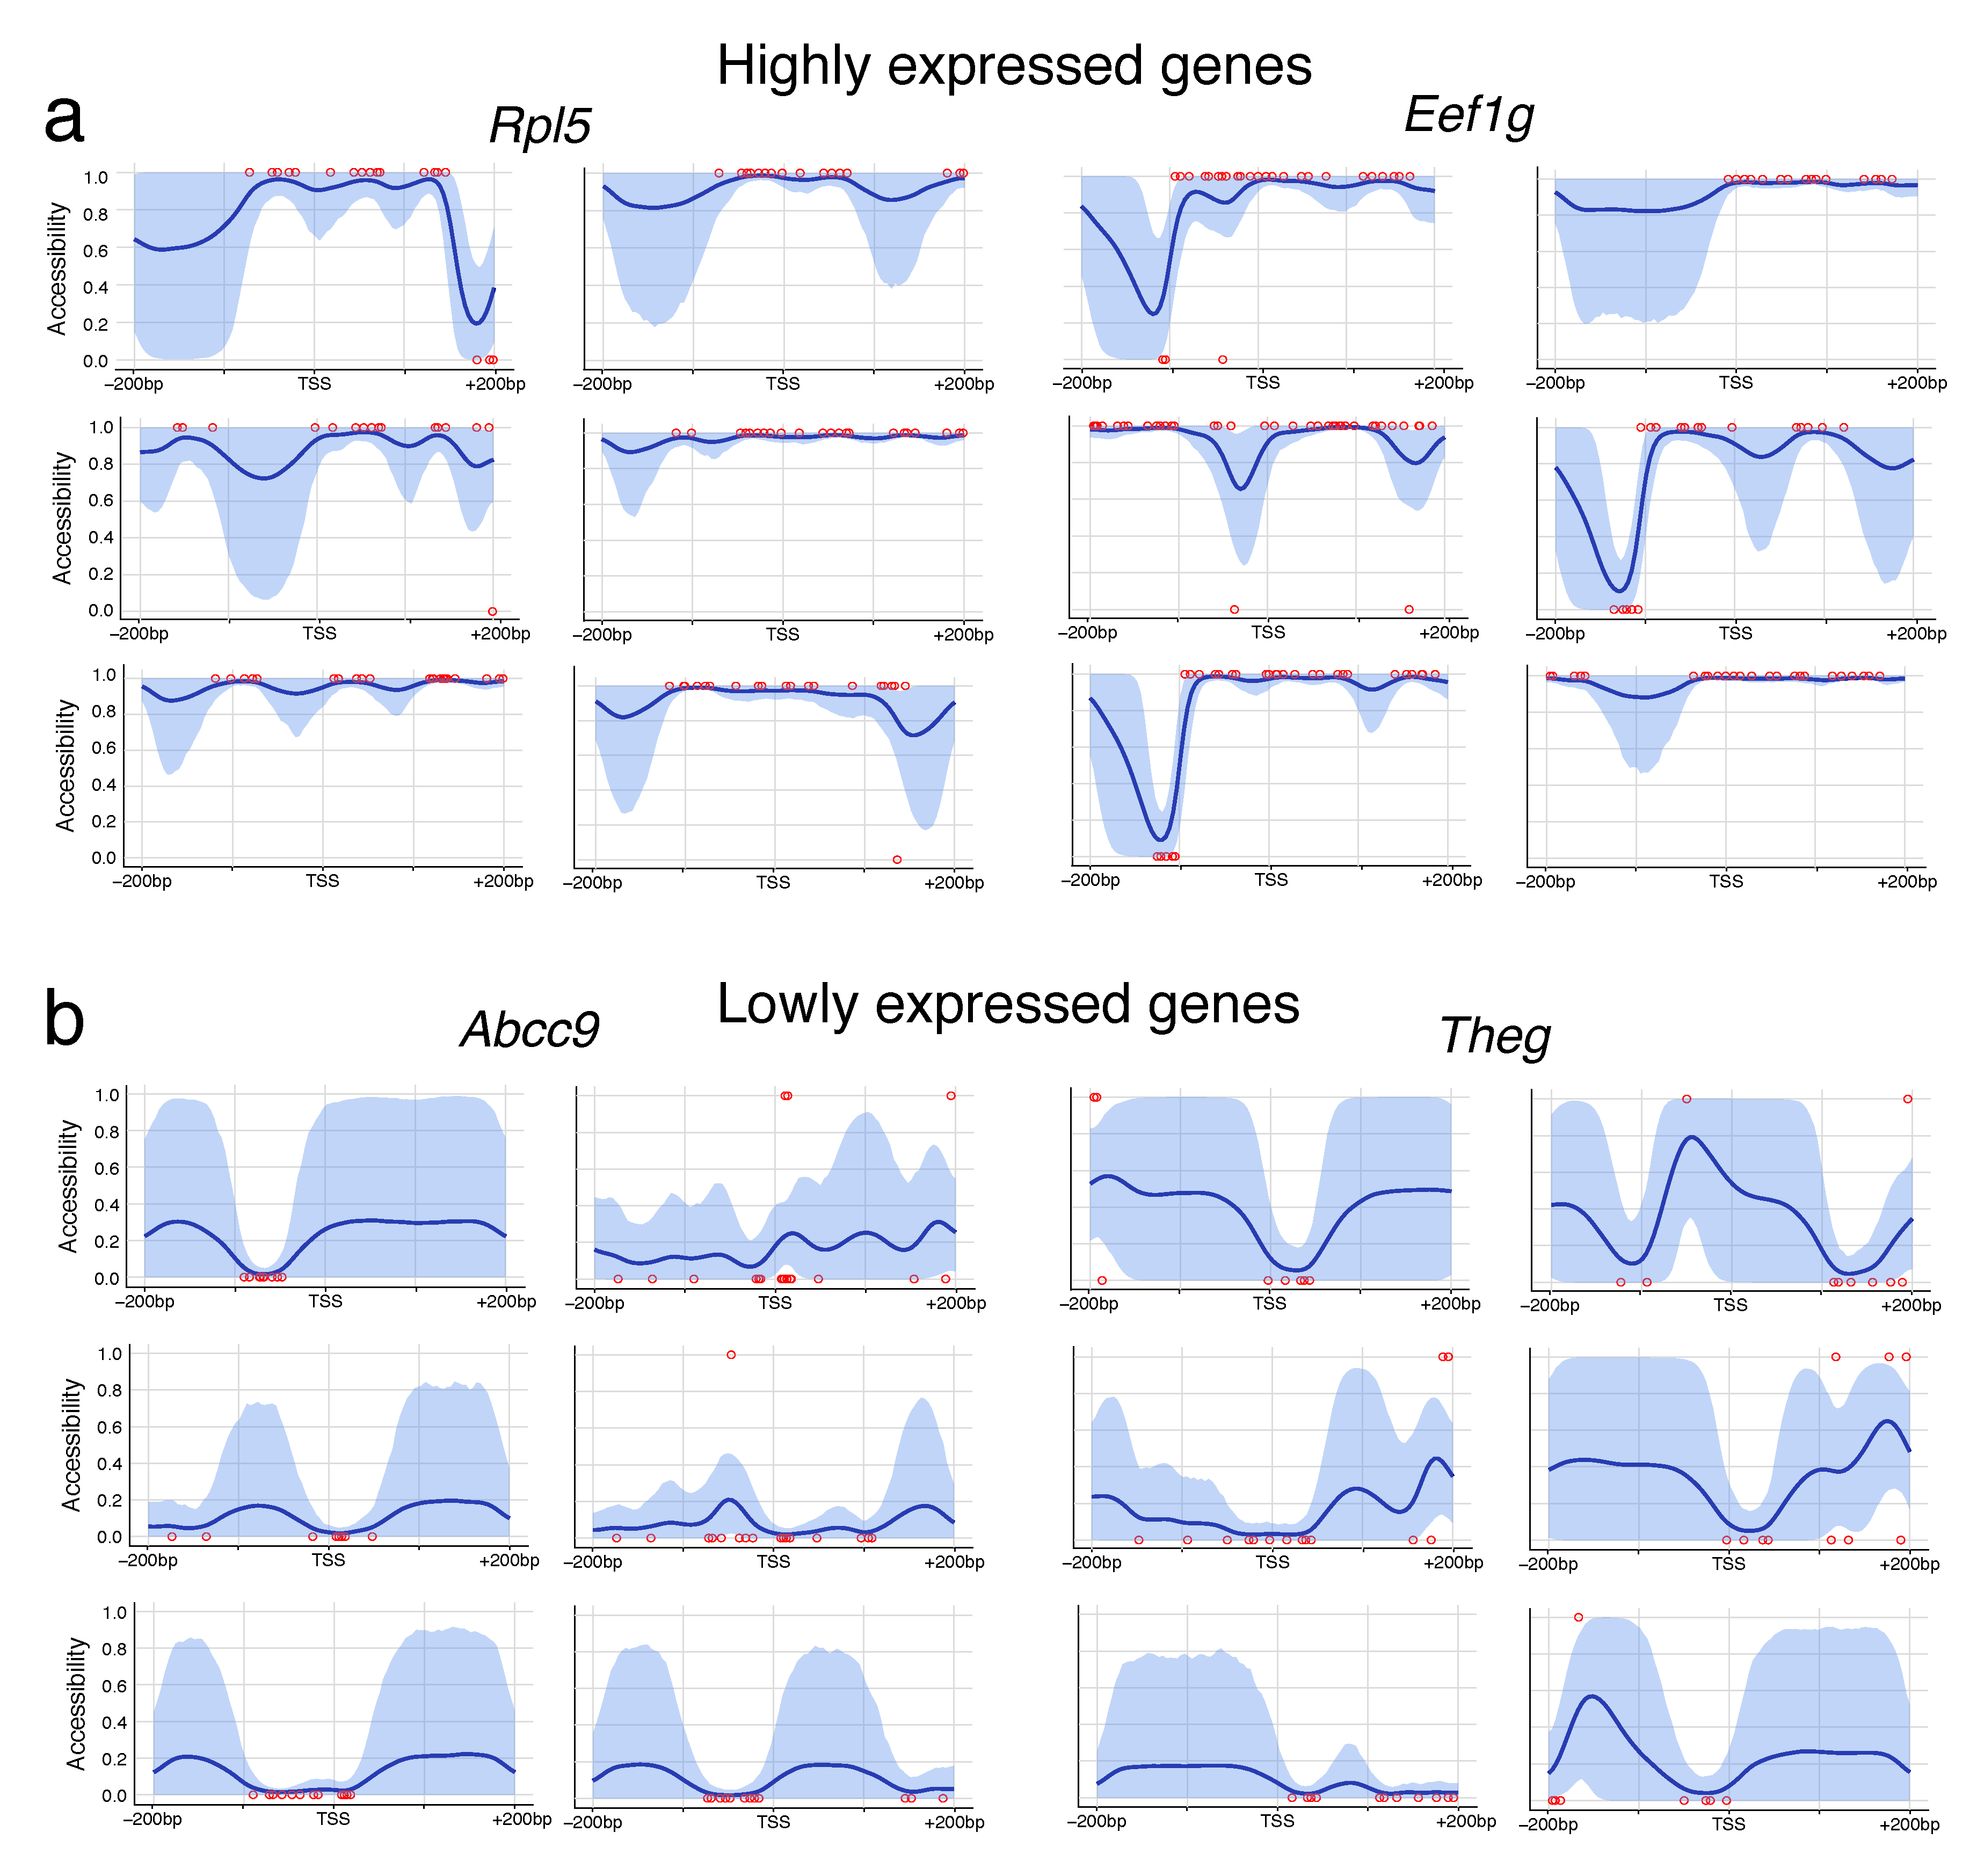
\includegraphics[width=0.9\linewidth]{scNMT_profiles_expr}
	\caption[]{}
	\label{fig:scnmt_profiles_highexpr}
\end{figure}

Next, we attempted at linking the heterogeneity in chromatin accessibility profiles with the variability in RNA expression.\\
A challenge of this augmented representation is how to find a one-dimensional statistic that summarises the heterogeneity across cells (as the variance statistic in conventional rates), which can be in turn correlated with summary statistics from the RNA expression. The approach we followed here is to cluster cells (per gene) based on the similarity of the accessibility profiles, using a finite mixture model with an expectation-maximisation algorithm. The optimal number of clusters was estimated using a Bayesian Information Criterion.\\
After model fitting, we considered the number of clusters as a proxy for accessibility heterogeneity, the rationale being that homogeneous genes will be grouped in a single cluster, while heterogeneous genes will contain a higher number of clusters.\\

\begin{figure}[H]
	\centering
	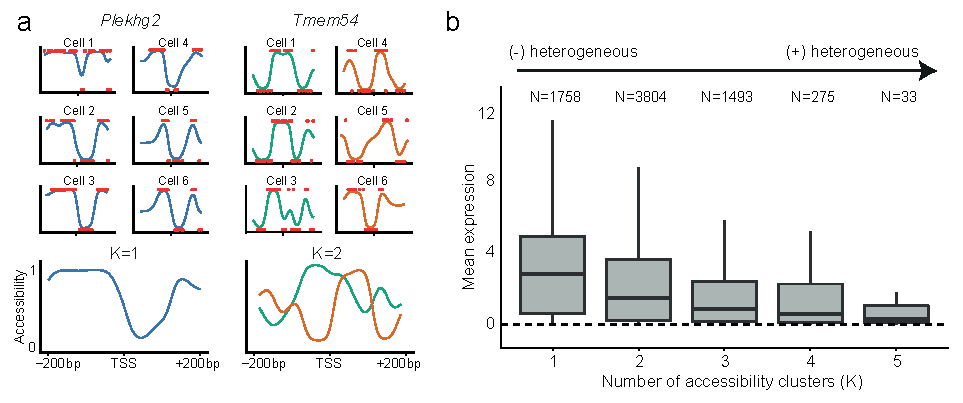
\includegraphics[width=0.9\linewidth]{scNMT_profiles_clusters}
	\caption[]{}
	\label{fig:scnmt_profiles_clusters}
\end{figure}

When relating the number of clusters to the gene expression, we observed that genes with homogeneous accessibility profiles (fewer clusters) were associated with higher average expression levels. Gene Ontology enrichment analysis suggests that this cluster is enriched by genes with houseekeping functions, which are known to display more conserved epigenetic features \cite{She2009}.\\
In contrast, genes with heterogeneous accessibility (multiple clusters) were associated with lower expression levels and were enriched for bivalent domains, containing both active H3K4me3 and repressive H3K27me3 histone marks. As reported in previous studies, bivalent chromatin is normally associated with lowly-expressed genes that are poised for activation upon cell differentiation, thus playing a fundamental role in pluripotency and development \cite{Vastenhouw2012,Bernstein2006}

\begin{figure}[H]
	\centering
	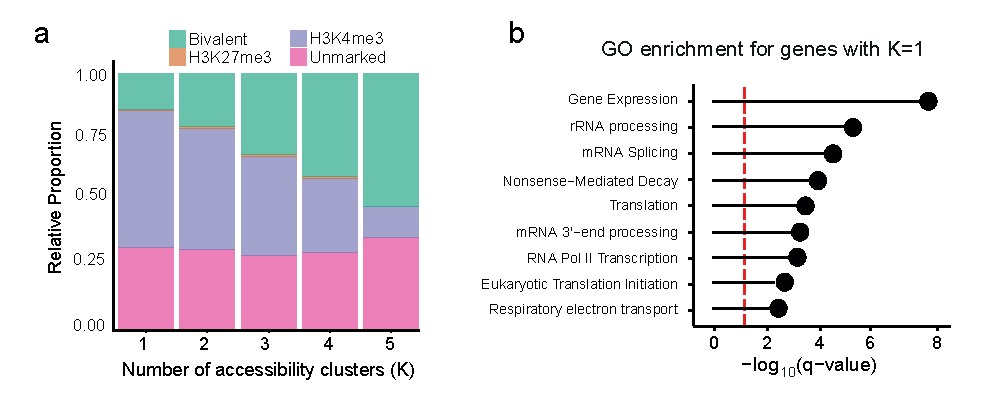
\includegraphics[width=0.9\linewidth]{scNMT_profiles_clusters2}
	\caption[]{}
	\label{fig:scnmt_profiles_clusters2}
\end{figure}




% \begin{figure}[H]
% 	\centering
% 	\includegraphics[width=0.9\linewidth]{scNMT_profiles_clusters_examples}
% 	\caption[]{}
% 	\label{fig:scnmt_profiles_clusters_examples}
% \end{figure}

In conclusion, we have shown that the use of non-linear methods for summarising NOMe-seq accessibility data can yield novel insights into the chromatin organisation, nucleosome positioning and the consequent regulation of gene expression. Yet, we acknowledge that this novel methodology needs to be further validated using other data sets, and some improvements need to be implemented in order to ensure that robust biological signal can be extracted from single-cell studies. First, the use of faster inference frameworks, which has been implemented in the new version of the software \cite{Kapourani2018}. Second, the method requires a large number of measurements for an accurate regression. In this study we used relatively lenient thresholds and only $\approx$25\% genes passed coverage filtering. An attempt to improve this could be the use of Bayesian methods that simultaneously cluster and fit the regression model, effectively leveraging information about the similarity between individual cells \cite{Kapourani2018b}. Finally, one could aim at learning a joint model with DNA methylation and chromatin accessiblity to provide an extra layer of multi-modal information.


\subsection{Characterisation of epigenome dynamics along a developmental trajectory}
The use of single-cell technologies has permitted the unbiased study of continuous trajectories by computationally reconstructing the \textit{pseudotemporal} dynamics from the molecular profiles \cite{Trapnell2014,Haghverdi2016,Saelens2018}. A novel opportunity unveiled by the introduction of single-cell multi-modal technologies is the study of epigenetic dynamics along pseudotime trajectories infered from the transcriptome.\\

To explore this idea, we applied a diffusion pseudotime method from the \textit{destiny} package\cite{Haghverdi2016}, using the RNA expression of the 500 genes with highest biological overdispersion, as estimated by the \textit{scran} package \cite{Lun2016}. The resulting first diffusion component was used to reconstruct a pseudotemporal ordering of cells from pluripotent to differentiated states:

\begin{figure}[H]
	\centering
	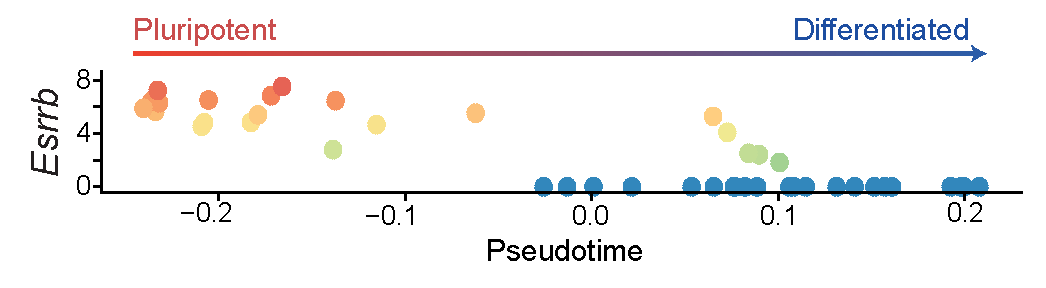
\includegraphics[width=0.9\linewidth]{scNMT_pseudotime}
	\caption[]{}
	\label{fig:scnmt_pseudotime}
\end{figure}


Next, we aimed at identifying genes with coordinated changes in the promoter accessibility and position of the cell in the trajectory using Spearman's rank coefficient test. This identified 15 significant genes, most of them showing a positive coefficient linked to a decrease in chromatin accessibility along the trajectory.

\begin{figure}[H]
	\centering
	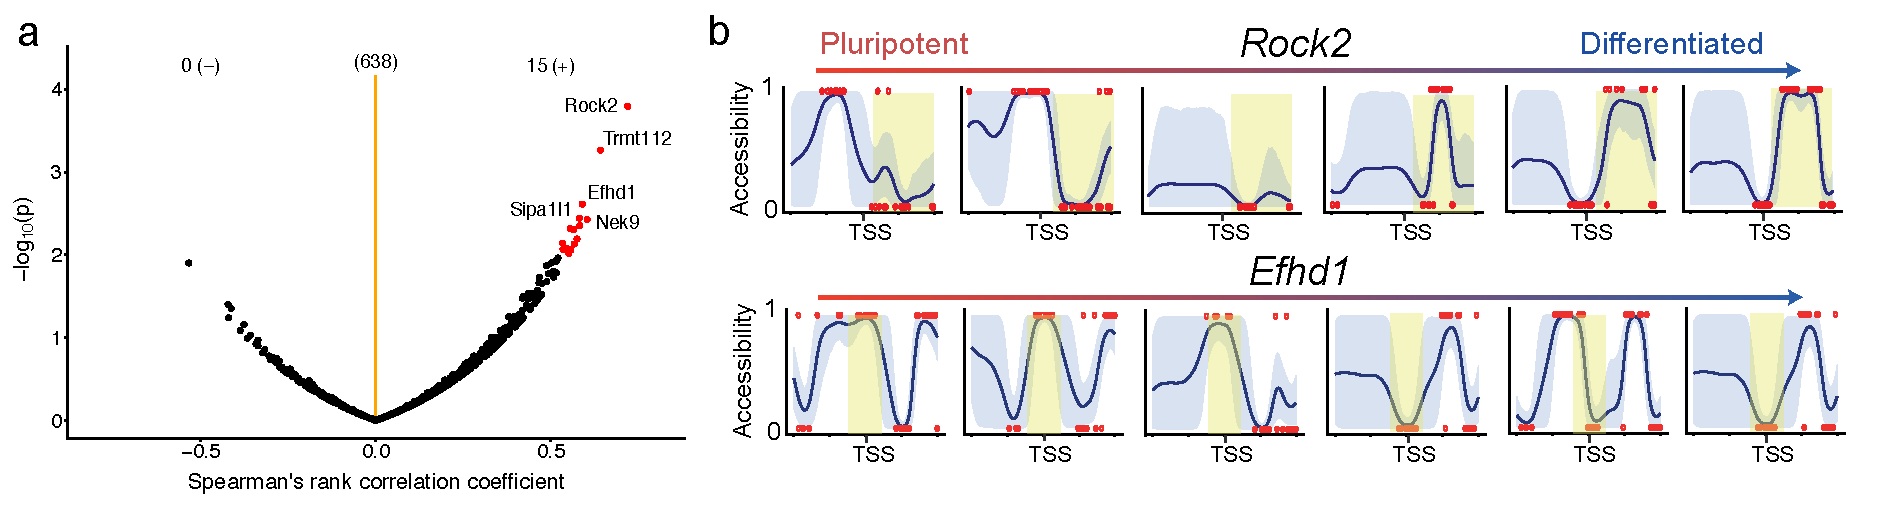
\includegraphics[width=0.9\linewidth]{scNMT_pseudotime_correlation}
	\caption[]{}
	\label{fig:scnmt_pseudotime_correlation}
\end{figure}

%(COPIED) Finally, we investigated whether dynamic changes in the coupling between the epigenetic layers are observed along the differentiation trajectory. To this end, we plotted methylation- accessibility correlation coefficients (as calculated in Fig. 2a) against pseudotime, which revealed an increasing negative correlation coefficient between DNA methylation and accessi- bility in practically all genomic contexts (Fig. 5c). Notably, this suggests that the coupling between the epigenetic layers increases as cells commit to downstream lineages, which could be an important step in lineage priming. Importantly, this analysis was made possible by the continuous nature of the single-cell pseudotime ordering and the ability to profile the three molecular layers and highlights the utility of such parallel single-cell techniques.


\begin{figure}[H]
	\centering
	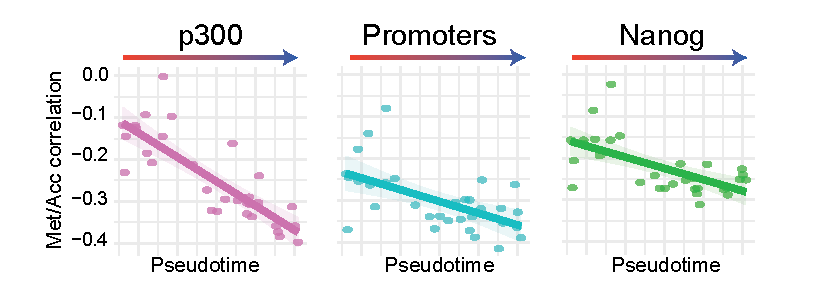
\includegraphics[width=0.9\linewidth]{scNMT_pseudotime_coupling}
	\caption[]{}
	\label{fig:scnmt_pseudotime_coupling}
\end{figure}

\section{Open perspectives}

Multi-modal sequencing technologies are becoming rapidly available. Yet, compared to scRNA-seq technologies, the field still is at an early stage amd numerous developments are expected to occur in the next years. These are lines of research that we are considering to improve scNMT-seq:

\begin{itemize}

	\item \textbf{Scalability}. scRNA-seq protocols are reaching the astonishing numbers of milions of cells per experiment, compared to the limited cell numbers achieved in multi-modal experiments \cite{Cao2019,Cao2018,Guo2017}. As in scRNA-seq, the maturation of multi-modal techniques will have a trade-off between sensitivity and scalability \cite{Chappell2018}. Under the assumption that epigenetic regulation is more strongly driven by local process compared to global interactions\cite{XX}, we emphasise the importance of obtaining high-resolution measurements as provided by scNMT-seq. Hence, effort should be placed on making this comprehensive technology more scalable, which can be achieved in the short term by a series of technical improvements.\\
	First, barcodes are currently added at the end of the protocol, which limits a single experiment to the size of the plate (typically 96 cells). As in droplet-based methods or combinatorial indexing methods, adding the barcodes at the start of the protocol would enable the simultaneous processing of multiple pools of cells \cite{droplet,sci-met}.
	Similarly, the physical separation of mRNA from genomic DNA is also carried out at the start of the protocol and individually for each cell. Given that it is a time-consuming and expensive process, this step should also be performed after pooling.\\
	Finally, sequencing costs are expected to decrease (even faster than predicted by Moore's law) \cite{Svensson2018}. Yet, the generation of scNMT-seq libraries remain inexorably more expensive than any scRNA-seq technology. Hence, efforts to decrease the library size by a pre-selection of the genetic material might be indispensable. Examples of such strategies are the digestion by restriction enzymes as in RRBBS \cite{Guo2013}, an initial round of ATAC protocol to select open chromatin \cite{Spektor2018}, 
	 	%this is a non-sequitur - it is high sequencing costs (not library prep costs) you mean to be talking about here

	\item \textbf{Imputation of missing epigenetic data}. Because of the low amounts of starting material, single-cell methylation protocols are limited by incomplete CpG coverage \cite{Angermueller2017}. These becomes even more pronounced in scNMT-seq where almost $\approx$ 50\% of CpG dinucleotides are removed to avoid technical biases (see \Cref{section:scnmt_coverage}). Nonetheless, as discussed in \Cref{section:scnmt_protocol}, an important advantage of bisulfite approaches is that missing data can be easily discriminated from inaccessible chromatin. Therefore, the imputation of DNA methylation data will be a critical step to enable genome-wide analysis.\\
	Most of the methods developed for bulk data are unsuccesful because they do not account for cell-to-cell variability \cite{Angermueller2017}. A successful single-cell strategy based on deep learning has been proposed (DeepCpG\cite{Angermueller2017}), but is a complex model that is difficult to train and does not scale to large studies. Faster and accurate Bayesian approaches have also been considered (Melissa \cite{Kapourani2018b}), albeit the model is restricted to small genomic annotations. An interesting direction would be to extend DeepCpG and Melissa to exploit the richness of information in the GpC accessibility data to refine the imputation of CpG measurements.

	\item \textbf{Adding more molecular layers}. The scNMT-seq protocol can be adapted both experimentally and computationally to profile additional molecular layers. From the computational side, one could exploit the sequence information in the libraries to infer copy number variation or single nucleotide variants \cite{Poirion2018,Fan2018,McCarthy2018,Enge2017}. This approach has been successful at dealineating the clonal substructure of somatic tissues and at tracking mutational signatures in cancer tissues.\\
	In addition, the full length transcript information enables the quantification of splice variants\cite{Huang2017}, allele-specific fractions\cite{Deng2014} and RNA velocity information \cite{LaManno2018}

	% Stephen: TF binding using https://doi.org/10.1101/538553 histone modifications using https://doi.org/10.1101/568915 - both in theory could be combined with some future NMTseq

	\item \textbf{Denoising}. The readouts from bisulfite sequencing are very sensitive \cite{XX}. However, in scNMT-seq the CGC positions (27\%) suffer from off-target effects of the GpC methylase \cite{Kelly2012}. In this work we have excluded those measurements to avoid undesired technical variation. Yet, no attempts have been carried to quantify this effect. If small enough, one could denoise the resulting CpG measurements by machine learning techniques that use sequence context information and pool information across cells.

	\item \textbf{Long reads}. The scNMT-seq libraries that were generated for this study contained short reads (???) that do not provide sufficient information about the regional context of the individual DNA molecule. By sequencing NOMe-seq libraries with long-read nanopore sequencing technology \cite{Lee2018} showed that one can obtain phased methyation and chromatin accessibility measurements and structural changes from a single assay. This approach could potentially unveil a more comprehensive understanding of the epigenome dynamics and its regulatory role on RNA expression.
		% Stephen: you could do the same with using SNPs to assign reads to alleles (e.g. in f1 mice)

\end{itemize}



